% !TEX root = ../multivar-notes.tex
\section{Integrals}
\subsection{Riemann Integral in $\R^n$}
\subsubsection*{March 7, 2019}
Goal: calculate a "total amount" from a "density function" defined over a region in $\R^n$. In order for this to work, we set two stipulations: 
\begin{itemize}
	\item the region is a bounded subset of $\R^n$
	\item the density function is a bounded function $f : \R^n \to \R$
\end{itemize}
Just as in BC Calculus, the idea is to refine a discrete problem by taking a limit. 

Example: 
\[U \subseteq \R^2\qquad U = \mtrx{0,3}\times \mtrx{0,2}\]
\[f : \R^2 \to \R \quad \text{is a density function}\]
\begin{center}
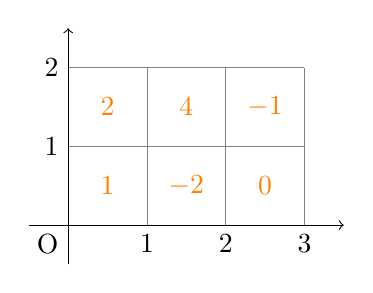
\begin{tikzpicture}
\draw[help lines,step=1] (0,0) grid (3,2);
\node[anchor=north east] at (0,0) {O};
\foreach \x in {1,2,3}
 \node[anchor=north] at (\x,0) {\x};
\foreach \y in {1,2}
 \node[anchor=east] at (0,\y) {\y};
 
\draw[->] (-0.5,0) -- (3.5,0);
\draw[->] (0,-0.5) -- (0,2.5);
\node[color=orange] at (0.5,0.5) {$1$};
\node[color=orange] at (1.5,0.5) {$-2$};
\node[color=orange] at (2.5,0.5) {$0$};
\node[color=orange] at (0.5,1.5) {$2$};
\node[color=orange] at (1.5,1.5) {$4$};
\node[color=orange] at (2.5,1.5) {$-1$};

\end{tikzpicture}

Total amount: \boxed{$4$}
\end{center}

If we refine the grid (let the number of grid squares go to infinity), we can consider this problem for a function $f(x,y)$, for example $f(x,y)=2x+y^2$. If this is the density on $U$, what is the amount now? 

\begin{center}
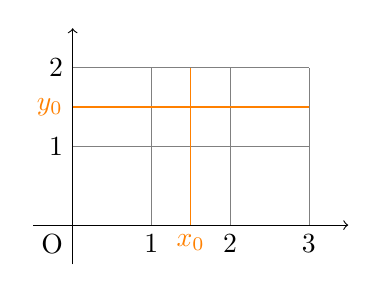
\begin{tikzpicture}
\draw[help lines,step=1] (0,0) grid (3,2);
\node[anchor=north east] at (0,0) {O};
\foreach \x in {1,2,3}
 \node[anchor=north] at (\x,0) {\x};
\foreach \y in {1,2}
 \node[anchor=east] at (0,\y) {\y};
 
\draw[->] (-0.5,0) -- (3.5,0);
\draw[->] (0,-0.5) -- (0,2.5);
\draw[-,color=orange] (1.5,0) -- (1.5,2);
\node[anchor=north,color=orange] at (1.5,0) {$x_0$};
\draw[-,color=orange] (0,1.5) -- (3,1.5);
\node[anchor=east,color=orange] at (0,1.5) {$y_0$};
\end{tikzpicture}
\end{center}
Let us, for example, hold the $x$-value constant at $x=x_0$. With the $x$-value held constant, we have now a function $h(y)=f(x_0,y)=2x_0+y^2$. We can then calculate the "total amount" on the vertical segment from $(x_0,0)$ to $(x_0,2)$. 
\begin{align*}
	&\hphantom{=}\int_0^2 f(x_0,y) dy \\
	&= \int_0^2 2x_0 + y^2 dy \\
	&= 2x_0y+\frac{1}{3}y^3 \Bigr\rvert_0^2 \\
	&= 4x_0+\frac{8}{3}
\end{align*}

Finally, the total amount over $U$ is obtained by integrating over the remaining $x$-variable: 
\[\int_{x=3}^3 4x_0 + \frac{8}{3} dx_0 = 2x_0^2 + \frac{8}{3} x_0 \Bigr\rvert_0^3=18+\frac{8}{3}3=26\]

This should be the same result as when we "go horizontally" first: 
\[\int_{y=0}^2\left(\int_{x=0}^32x+y^2 dx\right)dy=\int_{0}^2\left(x^2+xy^2\Bigr\rvert_0^3\right)dy=\int_0^2 9+3y\ dy=9y+y^3 \Bigr\rvert_0^2 =18+8=26\]

Intuitively, the following \ul{should} make sense: 
\begin{align*}
	\int_{[a,b]\times[c,d]} f(x,y) \left| d^2(x,y)\right| &=\int_a^b\System{\int_c^d f(x,y) dy}dx \\
	&=\int_c^d\System{\int_a^b f(x,y) dx}dy
\end{align*}
This (as well as its higher-dimensional analogs) is called \ul{Fubini's Theorem}. 

We can use these ideas without much complication to consider other types of regions:
\[\frac{x}{3}+\frac{y}{2}=1\]
\begin{center}
	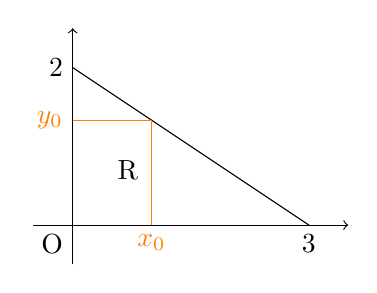
\begin{tikzpicture}
\node[anchor=north east] at (0,0) {O};
\foreach \x in {3}
 \node[anchor=north] at (\x,0) {\x};
\foreach \y in {2}
 \node[anchor=east] at (0,\y) {\y};
 
\draw[->] (-0.5,0) -- (3.5,0);
\draw[->] (0,-0.5) -- (0,2.5);
\draw[-] (0,2) -- (3,0);
\node[] at (0.7,0.7) {R};
\draw[-,color=orange] (1,4/3) -- (1,0);
\node[anchor=north,color=orange] at (1,0) {$x_0$};
\draw[-,color=orange] (0,4/3) -- (1,4/3);
\node[anchor=east,color=orange] at (0,4/3) {$y_0$};
\end{tikzpicture}
\end{center}